\documentclass[dvipsnames]{beamer}
\input{mybeamerdefs}
\title{MRI Simulator Notes}
\author{Liam}
\date{\today}

\begin{document}

\begin{frame}
\maketitle
\end{frame}

\begin{frame}{Tasks}
\begin{itemize}
\item I ran the 2DFT simulation + reconstruction using single ems placed at different locations to look at the point-spread function.
\item I rewrote some pulse sequence functions to incorporate a user-specified TR and TE and ran the 2DFT simulation + reconstruction using the parameters Chuck suggested.
\item I looked at the effect on the total memory usage of increasing the number of ems and the pulse sequence length.
\end{itemize}
\end{frame}

\section{2DFT point-spread function}

\begin{frame}{Summary}
\begin{itemize}
\item All the same simulation parameters as in 2019-12-10, which I found to be T1 = 10 ms, T2 = 10 ms, TE = 1 ms, TR = 53 ms.
\item I wanted to look at the ``asymmetric blurring" I noted in 2019-12-10. Chuck hypothesized it was due to the sum of multiple point-spread functions.
\item I placed an em with an offset in $x$, then the negative of the offset, and the same for $y$, to see if the point-spread function is simply reflected about the origin for these reflected offsets.
\end{itemize}
\end{frame}

\begin{frame}
\begin{center}
\includegraphics[width=\textwidth]{{reconstruction_x-0.5_y-0.0}.pdf}
\end{center}
\end{frame}

\begin{frame}
\begin{center}
\includegraphics[width=\textwidth]{{reconstruction_x-minus-0.5_y-0.0}.pdf}
\end{center}
\end{frame}

\begin{frame}
\begin{center}
\includegraphics[width=\textwidth]{{reconstruction_x-0.0_y-0.5}.pdf}
\end{center}
\end{frame}

\begin{frame}
\begin{center}
\includegraphics[width=\textwidth]{{reconstruction_x-0.0_y-minus-0.5}.pdf}
\end{center}
\end{frame}

\begin{frame}{Comments}
\begin{itemize}
\item The point-spread function itself appears to be asymmetric. Not sure what this means regarding the simulation and/or reconstruction. Is this typical in MR?
\item By eye, the point-spread function is reflected when the $x$ position is reflected; the same is untrue of $y$. $y$ is the phase-encoding direction, and the k-space lines are scanned starting with maximum positive $k_y$. Could this have something to do with it?
\end{itemize}
\end{frame}

\section{2DFT simulation with better parameters}

\begin{frame}{Summary}
\begin{itemize}
\item I redid the simulations of the previous section with the parameters T1 = 100 ms, T2 = 10 ms, TE = 4 ms, TR = 100 ms.
\end{itemize}
\end{frame}

\begin{frame}
\begin{center}
\includegraphics[width=\textwidth]{{reconstruction_T1-100ms_T2-10ms_TE-4ms_TR-100ms_x-0.5_y-0.0}.pdf}
\end{center}
\end{frame}

\begin{frame}
\begin{center}
\includegraphics[width=\textwidth]{{reconstruction_T1-100ms_T2-10ms_TE-4ms_TR-100ms_x-minus-0.5_y-0.0}.pdf}
\end{center}
\end{frame}

\begin{frame}
\begin{center}
\includegraphics[width=\textwidth]{{reconstruction_T1-100ms_T2-10ms_TE-4ms_TR-100ms_x-0.0_y-0.5}.pdf}
\end{center}
\end{frame}

\begin{frame}
\begin{center}
\includegraphics[width=\textwidth]{{reconstruction_T1-100ms_T2-10ms_TE-4ms_TR-100ms_x-0.0_y-minus-0.5}.pdf}
\end{center}
\end{frame}

\begin{frame}{Comments}
\begin{itemize}
\item The reconstructions are similar to those of the previous section.
\item There is more blurring for $(x,y) = (0.0,0.5)$ than in the previous section.
\item The point-spread function is reflected in $x$ but not in $y$ when the em position is reflected, again like the previous section.
\end{itemize}
\end{frame}

\section{Memory usage}

\begin{frame}{Summary}
\begin{itemize}
\item I instantiated a simulation object \texttt{Sim} with a variable number of ems (did not run simulation). I recorded the memory usage of this instantiation command. The plots on the next slides show the results.
\item I ran the simulation with a fixed number of ems and varied the pulse length. To save time, I took a single time step for each pulse. I recorded the memory usage of the \texttt{run\_sim} command. Changing the pulse length only changes the memory usage of the Pulse instantiation command, not the \texttt{Sim} instantiation command nor the \texttt{run\_sim} command.
\end{itemize}
\end{frame}

\begin{frame}{Liam's Macbook}
\begin{center}
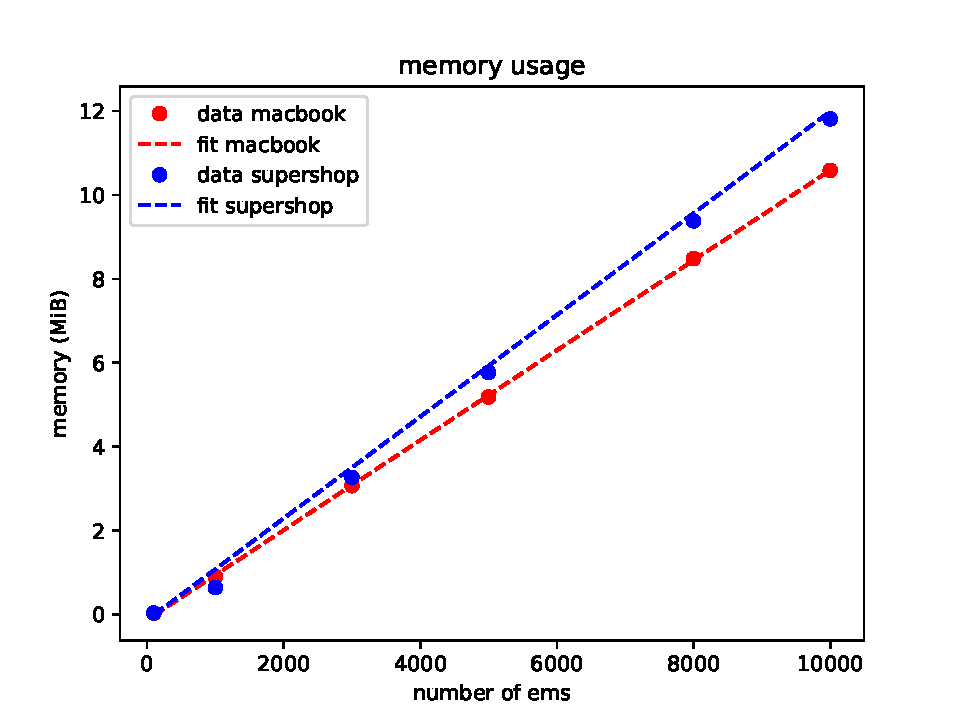
\includegraphics[height=0.8\textheight]{mem_num_ems}
1.12 kB per em.
\end{center}
\end{frame}

\begin{frame}{Supershop}
\begin{center}
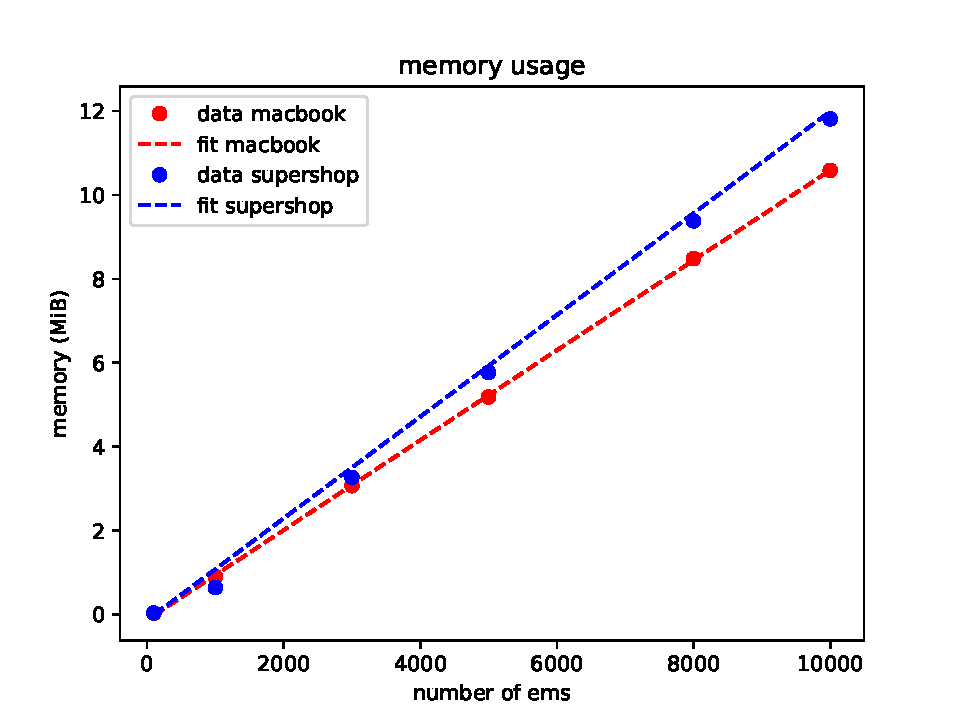
\includegraphics[height=0.8\textheight]{mem_num_ems}
1.12 kB per em.
\end{center}
\end{frame}

\end{document}